\documentclass[twoside]{book}

% Packages required by doxygen
\usepackage{fixltx2e}
\usepackage{calc}
\usepackage{doxygen}
\usepackage[export]{adjustbox} % also loads graphicx
\usepackage{graphicx}
\usepackage[utf8]{inputenc}
\usepackage{makeidx}
\usepackage{multicol}
\usepackage{multirow}
\PassOptionsToPackage{warn}{textcomp}
\usepackage{textcomp}
\usepackage[nointegrals]{wasysym}
\usepackage[table]{xcolor}

% Font selection
\usepackage[T1]{fontenc}
\usepackage[scaled=.90]{helvet}
\usepackage{courier}
\usepackage{amssymb}
\usepackage{sectsty}
\renewcommand{\familydefault}{\sfdefault}
\allsectionsfont{%
  \fontseries{bc}\selectfont%
  \color{darkgray}%
}
\renewcommand{\DoxyLabelFont}{%
  \fontseries{bc}\selectfont%
  \color{darkgray}%
}
\newcommand{\+}{\discretionary{\mbox{\scriptsize$\hookleftarrow$}}{}{}}

% Page & text layout
\usepackage{geometry}
\geometry{%
  a4paper,%
  top=2.5cm,%
  bottom=2.5cm,%
  left=2.5cm,%
  right=2.5cm%
}
\tolerance=750
\hfuzz=15pt
\hbadness=750
\setlength{\emergencystretch}{15pt}
\setlength{\parindent}{0cm}
\setlength{\parskip}{3ex plus 2ex minus 2ex}
\makeatletter
\renewcommand{\paragraph}{%
  \@startsection{paragraph}{4}{0ex}{-1.0ex}{1.0ex}{%
    \normalfont\normalsize\bfseries\SS@parafont%
  }%
}
\renewcommand{\subparagraph}{%
  \@startsection{subparagraph}{5}{0ex}{-1.0ex}{1.0ex}{%
    \normalfont\normalsize\bfseries\SS@subparafont%
  }%
}
\makeatother

% Headers & footers
\usepackage{fancyhdr}
\pagestyle{fancyplain}
\fancyhead[LE]{\fancyplain{}{\bfseries\thepage}}
\fancyhead[CE]{\fancyplain{}{}}
\fancyhead[RE]{\fancyplain{}{\bfseries\leftmark}}
\fancyhead[LO]{\fancyplain{}{\bfseries\rightmark}}
\fancyhead[CO]{\fancyplain{}{}}
\fancyhead[RO]{\fancyplain{}{\bfseries\thepage}}
\fancyfoot[LE]{\fancyplain{}{}}
\fancyfoot[CE]{\fancyplain{}{}}
\fancyfoot[RE]{\fancyplain{}{\bfseries\scriptsize Generated by Doxygen }}
\fancyfoot[LO]{\fancyplain{}{\bfseries\scriptsize Generated by Doxygen }}
\fancyfoot[CO]{\fancyplain{}{}}
\fancyfoot[RO]{\fancyplain{}{}}
\renewcommand{\footrulewidth}{0.4pt}
\renewcommand{\chaptermark}[1]{%
  \markboth{#1}{}%
}
\renewcommand{\sectionmark}[1]{%
  \markright{\thesection\ #1}%
}

% Indices & bibliography
\usepackage{natbib}
\usepackage[titles]{tocloft}
\setcounter{tocdepth}{3}
\setcounter{secnumdepth}{5}
\makeindex

% Hyperlinks (required, but should be loaded last)
\usepackage{ifpdf}
\ifpdf
  \usepackage[pdftex,pagebackref=true]{hyperref}
\else
  \usepackage[ps2pdf,pagebackref=true]{hyperref}
\fi
\hypersetup{%
  colorlinks=true,%
  linkcolor=blue,%
  citecolor=blue,%
  unicode%
}

% Custom commands
\newcommand{\clearemptydoublepage}{%
  \newpage{\pagestyle{empty}\cleardoublepage}%
}

\usepackage{caption}
\captionsetup{labelsep=space,justification=centering,font={bf},singlelinecheck=off,skip=4pt,position=top}

%===== C O N T E N T S =====

\begin{document}

% Titlepage & ToC
\hypersetup{pageanchor=false,
             bookmarksnumbered=true,
             pdfencoding=unicode
            }
\pagenumbering{alph}
\begin{titlepage}
\vspace*{7cm}
\begin{center}%
{\Large Tratamento De Poligonos }\\
\vspace*{1cm}
{\large Generated by Doxygen 1.8.14}\\
\end{center}
\end{titlepage}
\clearemptydoublepage
\pagenumbering{roman}
\tableofcontents
\clearemptydoublepage
\pagenumbering{arabic}
\hypersetup{pageanchor=true}

%--- Begin generated contents ---
\chapter{R\+E\+A\+D\+ME}
\label{md__r_e_a_d_m_e}
\Hypertarget{md__r_e_a_d_m_e}
Projeto 1 -\/ Tratamento de Poligonos

primeiro projeto da segunda unidade da matéria D\+C\+A-\/1202. 
\chapter{Hierarchical Index}
\section{Class Hierarchy}
This inheritance list is sorted roughly, but not completely, alphabetically\+:\begin{DoxyCompactList}
\item \contentsline{section}{Point}{\pageref{class_point}}{}
\item \contentsline{section}{Poligono}{\pageref{class_poligono}}{}
\begin{DoxyCompactList}
\item \contentsline{section}{Retangulo}{\pageref{class_retangulo}}{}
\end{DoxyCompactList}
\end{DoxyCompactList}

\chapter{Class Index}
\section{Class List}
Here are the classes, structs, unions and interfaces with brief descriptions\+:\begin{DoxyCompactList}
\item\contentsline{section}{\mbox{\hyperlink{class_point}{Point}} \\*é usada para criar Pontos em um Plano Bidimensional }{\pageref{class_point}}{}
\item\contentsline{section}{\mbox{\hyperlink{class_poligono}{Poligono}} \\*é usado para representar polígonos convexos }{\pageref{class_poligono}}{}
\item\contentsline{section}{\mbox{\hyperlink{class_retangulo}{Retangulo}} \\*é uma subclasse da Class \mbox{\hyperlink{class_poligono}{Poligono}} }{\pageref{class_retangulo}}{}
\end{DoxyCompactList}

\chapter{File Index}
\section{File List}
Here is a list of all files with brief descriptions\+:\begin{DoxyCompactList}
\item\contentsline{section}{\mbox{\hyperlink{main_8cpp}{main.\+cpp}} }{\pageref{main_8cpp}}{}
\item\contentsline{section}{\mbox{\hyperlink{point_8cpp}{point.\+cpp}} }{\pageref{point_8cpp}}{}
\item\contentsline{section}{\mbox{\hyperlink{point_8h}{point.\+h}} }{\pageref{point_8h}}{}
\end{DoxyCompactList}

\chapter{Class Documentation}
\hypertarget{class_point}{}\section{Point Class Reference}
\label{class_point}\index{Point@{Point}}


The \mbox{\hyperlink{class_point}{Point}} class é usada para criar Pontos em um Plano Bidimensional.  




{\ttfamily \#include $<$point.\+h$>$}

\subsection*{Public Member Functions}
\begin{DoxyCompactItemize}
\item 
\mbox{\hyperlink{class_point_a2e9cc55fe05ce04457997f4f19aaa28d}{Point}} (float mx=0.\+0, float my=0.\+0)
\begin{DoxyCompactList}\small\item\em \mbox{\hyperlink{class_point}{Point}} é o Contrutor com Argumentos da Classe. \end{DoxyCompactList}\item 
\mbox{\hyperlink{class_point_a395fa04b4ec126b66fc053f829a30cc1}{$\sim$\+Point}} ()
\item 
\mbox{\hyperlink{class_point_af0c0f20db1616447bc78184ed537ef6e}{Point}} (const \mbox{\hyperlink{class_point}{Point}} \&p)
\begin{DoxyCompactList}\small\item\em \mbox{\hyperlink{class_point}{Point}} é o Construtor de Copia. \end{DoxyCompactList}\item 
void \mbox{\hyperlink{class_point_acee4acaa1d515e9973145f977e500fe6}{setX}} (float mx)
\begin{DoxyCompactList}\small\item\em setX Função que define a coordenada X; \end{DoxyCompactList}\item 
void \mbox{\hyperlink{class_point_a756b3f64d961a5059302f42e1fcf2332}{setY}} (float my)
\begin{DoxyCompactList}\small\item\em setY Função que define a coordenada Y; \end{DoxyCompactList}\item 
void \mbox{\hyperlink{class_point_afe2b937778d9fe5c135ab61de91271e9}{set\+XY}} (float mx, float my)
\begin{DoxyCompactList}\small\item\em set\+XY, Define em uma mesma função, as coordenadas X e Y; \end{DoxyCompactList}\item 
float \mbox{\hyperlink{class_point_a9aa94b8fd07296e64d304ef3750db113}{getX}} (void)
\begin{DoxyCompactList}\small\item\em getX Recupera a coordenada X do Ponto; \end{DoxyCompactList}\item 
float \mbox{\hyperlink{class_point_a2444daa96871c89614510bc4bfcd19ce}{getY}} (void)
\begin{DoxyCompactList}\small\item\em getY Recupera a coordenada Y do Ponto; \end{DoxyCompactList}\item 
\mbox{\hyperlink{class_point}{Point}} \mbox{\hyperlink{class_point_a9dbea84b07b0a8ec3bbb9e58b3d15899}{add}} (\mbox{\hyperlink{class_point}{Point}} p1)
\begin{DoxyCompactList}\small\item\em add é uma função que adiciona as coordenadas (x,y) do ponto com as coordenadas de um ponto P1(x1,y1) fornecido, armazenando o resultado nas coordenadas de um novo ponto. \end{DoxyCompactList}\item 
\mbox{\hyperlink{class_point}{Point}} \mbox{\hyperlink{class_point_a9cf2c53b0a4e6282a6712824bb4e9b00}{sub}} (\mbox{\hyperlink{class_point}{Point}} p1)
\begin{DoxyCompactList}\small\item\em sub é uma função que subtrai as coordenadas (x,y) do ponto com as coordenadas de um ponto P1(x1,y1) fornecido, armazenando o resultado nas coordenadas de um novo ponto. \end{DoxyCompactList}\item 
float \mbox{\hyperlink{class_point_aa3005a9d97e2cb05624414973a214788}{norma}} (void)
\begin{DoxyCompactList}\small\item\em norma Calcula a distância do ponto a origem de coordenadas. \end{DoxyCompactList}\item 
void \mbox{\hyperlink{class_point_ad9676e36f3444534b609e3c68422239a}{translada}} (float a, float b)
\begin{DoxyCompactList}\small\item\em translada Translada o ponto (x,y) de (+a,+b), de modo que, após a execução do método, as coordenadas do ponto serão (x+a,y+b). \end{DoxyCompactList}\item 
void \mbox{\hyperlink{class_point_a7c50a40a930fb7f3adc0f8e7b60b7d79}{Imprime}} ()
\begin{DoxyCompactList}\small\item\em Imprime, Função que monstra na tela o ponto na forma (xpos,ypos);. \end{DoxyCompactList}\item 
void \mbox{\hyperlink{class_point_a5d756c4b1cf7aeeb49ac79ff8cd3d1e9}{Rot}} (float ang)
\begin{DoxyCompactList}\small\item\em Rot, Função que rotaciona o ponto em torno de um angulo. \end{DoxyCompactList}\end{DoxyCompactItemize}


\subsection{Detailed Description}
The \mbox{\hyperlink{class_point}{Point}} class é usada para criar Pontos em um Plano Bidimensional. 

\subsection{Constructor \& Destructor Documentation}
\mbox{\Hypertarget{class_point_a2e9cc55fe05ce04457997f4f19aaa28d}\label{class_point_a2e9cc55fe05ce04457997f4f19aaa28d}} 
\index{Point@{Point}!Point@{Point}}
\index{Point@{Point}!Point@{Point}}
\subsubsection{\texorpdfstring{Point()}{Point()}\hspace{0.1cm}{\footnotesize\ttfamily [1/2]}}
{\footnotesize\ttfamily Point\+::\+Point (\begin{DoxyParamCaption}\item[{float}]{mx = {\ttfamily 0.0},  }\item[{float}]{my = {\ttfamily 0.0} }\end{DoxyParamCaption})}



\mbox{\hyperlink{class_point}{Point}} é o Contrutor com Argumentos da Classe. 


\begin{DoxyParams}{Parameters}
{\em mx} & Paramentro para a Coordenada X \\
\hline
{\em my} & Paramentro para a Coordenada Y \\
\hline
\end{DoxyParams}
\mbox{\Hypertarget{class_point_a395fa04b4ec126b66fc053f829a30cc1}\label{class_point_a395fa04b4ec126b66fc053f829a30cc1}} 
\index{Point@{Point}!````~Point@{$\sim$\+Point}}
\index{````~Point@{$\sim$\+Point}!Point@{Point}}
\subsubsection{\texorpdfstring{$\sim$\+Point()}{~Point()}}
{\footnotesize\ttfamily Point\+::$\sim$\+Point (\begin{DoxyParamCaption}{ }\end{DoxyParamCaption})}

\mbox{\Hypertarget{class_point_af0c0f20db1616447bc78184ed537ef6e}\label{class_point_af0c0f20db1616447bc78184ed537ef6e}} 
\index{Point@{Point}!Point@{Point}}
\index{Point@{Point}!Point@{Point}}
\subsubsection{\texorpdfstring{Point()}{Point()}\hspace{0.1cm}{\footnotesize\ttfamily [2/2]}}
{\footnotesize\ttfamily Point\+::\+Point (\begin{DoxyParamCaption}\item[{const \mbox{\hyperlink{class_point}{Point}} \&}]{p }\end{DoxyParamCaption})}



\mbox{\hyperlink{class_point}{Point}} é o Construtor de Copia. 


\begin{DoxyParams}{Parameters}
{\em p} & é o Ponto que sera copiado \\
\hline
\end{DoxyParams}


\subsection{Member Function Documentation}
\mbox{\Hypertarget{class_point_a9dbea84b07b0a8ec3bbb9e58b3d15899}\label{class_point_a9dbea84b07b0a8ec3bbb9e58b3d15899}} 
\index{Point@{Point}!add@{add}}
\index{add@{add}!Point@{Point}}
\subsubsection{\texorpdfstring{add()}{add()}}
{\footnotesize\ttfamily \mbox{\hyperlink{class_point}{Point}} Point\+::add (\begin{DoxyParamCaption}\item[{\mbox{\hyperlink{class_point}{Point}}}]{p1 }\end{DoxyParamCaption})}



add é uma função que adiciona as coordenadas (x,y) do ponto com as coordenadas de um ponto P1(x1,y1) fornecido, armazenando o resultado nas coordenadas de um novo ponto. 


\begin{DoxyParams}{Parameters}
{\em p1} & é o ponto passado como parametro. \\
\hline
\end{DoxyParams}
\begin{DoxyReturn}{Returns}
a função retorna um ponto com as coordendas (x + p1.\+x, y + p1.\+y); 
\end{DoxyReturn}
\mbox{\Hypertarget{class_point_a9aa94b8fd07296e64d304ef3750db113}\label{class_point_a9aa94b8fd07296e64d304ef3750db113}} 
\index{Point@{Point}!getX@{getX}}
\index{getX@{getX}!Point@{Point}}
\subsubsection{\texorpdfstring{get\+X()}{getX()}}
{\footnotesize\ttfamily float Point\+::getX (\begin{DoxyParamCaption}\item[{void}]{ }\end{DoxyParamCaption})}



getX Recupera a coordenada X do Ponto; 

\begin{DoxyReturn}{Returns}
Valor da Coordenada X; 
\end{DoxyReturn}
\mbox{\Hypertarget{class_point_a2444daa96871c89614510bc4bfcd19ce}\label{class_point_a2444daa96871c89614510bc4bfcd19ce}} 
\index{Point@{Point}!getY@{getY}}
\index{getY@{getY}!Point@{Point}}
\subsubsection{\texorpdfstring{get\+Y()}{getY()}}
{\footnotesize\ttfamily float Point\+::getY (\begin{DoxyParamCaption}\item[{void}]{ }\end{DoxyParamCaption})}



getY Recupera a coordenada Y do Ponto; 

\begin{DoxyReturn}{Returns}
Valor da Coordenada y; 
\end{DoxyReturn}
\mbox{\Hypertarget{class_point_a7c50a40a930fb7f3adc0f8e7b60b7d79}\label{class_point_a7c50a40a930fb7f3adc0f8e7b60b7d79}} 
\index{Point@{Point}!Imprime@{Imprime}}
\index{Imprime@{Imprime}!Point@{Point}}
\subsubsection{\texorpdfstring{Imprime()}{Imprime()}}
{\footnotesize\ttfamily void Point\+::\+Imprime (\begin{DoxyParamCaption}{ }\end{DoxyParamCaption})}



Imprime, Função que monstra na tela o ponto na forma (xpos,ypos);. 

\mbox{\Hypertarget{class_point_aa3005a9d97e2cb05624414973a214788}\label{class_point_aa3005a9d97e2cb05624414973a214788}} 
\index{Point@{Point}!norma@{norma}}
\index{norma@{norma}!Point@{Point}}
\subsubsection{\texorpdfstring{norma()}{norma()}}
{\footnotesize\ttfamily float Point\+::norma (\begin{DoxyParamCaption}\item[{void}]{ }\end{DoxyParamCaption})}



norma Calcula a distância do ponto a origem de coordenadas. 

\begin{DoxyReturn}{Returns}
retorna a distância. 
\end{DoxyReturn}
\mbox{\Hypertarget{class_point_a5d756c4b1cf7aeeb49ac79ff8cd3d1e9}\label{class_point_a5d756c4b1cf7aeeb49ac79ff8cd3d1e9}} 
\index{Point@{Point}!Rot@{Rot}}
\index{Rot@{Rot}!Point@{Point}}
\subsubsection{\texorpdfstring{Rot()}{Rot()}}
{\footnotesize\ttfamily void Point\+::\+Rot (\begin{DoxyParamCaption}\item[{float}]{ang }\end{DoxyParamCaption})}



Rot, Função que rotaciona o ponto em torno de um angulo. 


\begin{DoxyParams}{Parameters}
{\em ang,angulo} & passado como paramentro. \\
\hline
\end{DoxyParams}
\mbox{\Hypertarget{class_point_acee4acaa1d515e9973145f977e500fe6}\label{class_point_acee4acaa1d515e9973145f977e500fe6}} 
\index{Point@{Point}!setX@{setX}}
\index{setX@{setX}!Point@{Point}}
\subsubsection{\texorpdfstring{set\+X()}{setX()}}
{\footnotesize\ttfamily void Point\+::setX (\begin{DoxyParamCaption}\item[{float}]{mx }\end{DoxyParamCaption})}



setX Função que define a coordenada X; 


\begin{DoxyParams}{Parameters}
{\em mx} & Parametro passado para a função SetX; \\
\hline
\end{DoxyParams}
\mbox{\Hypertarget{class_point_afe2b937778d9fe5c135ab61de91271e9}\label{class_point_afe2b937778d9fe5c135ab61de91271e9}} 
\index{Point@{Point}!set\+XY@{set\+XY}}
\index{set\+XY@{set\+XY}!Point@{Point}}
\subsubsection{\texorpdfstring{set\+X\+Y()}{setXY()}}
{\footnotesize\ttfamily void Point\+::set\+XY (\begin{DoxyParamCaption}\item[{float}]{mx,  }\item[{float}]{my }\end{DoxyParamCaption})}



set\+XY, Define em uma mesma função, as coordenadas X e Y; 


\begin{DoxyParams}{Parameters}
{\em mx} & Paramentro da coordenada x passado para a função Set\+XY; \\
\hline
{\em my} & Paramentro da coordenada y passada para a função Set\+XY; \\
\hline
\end{DoxyParams}
\mbox{\Hypertarget{class_point_a756b3f64d961a5059302f42e1fcf2332}\label{class_point_a756b3f64d961a5059302f42e1fcf2332}} 
\index{Point@{Point}!setY@{setY}}
\index{setY@{setY}!Point@{Point}}
\subsubsection{\texorpdfstring{set\+Y()}{setY()}}
{\footnotesize\ttfamily void Point\+::setY (\begin{DoxyParamCaption}\item[{float}]{my }\end{DoxyParamCaption})}



setY Função que define a coordenada Y; 


\begin{DoxyParams}{Parameters}
{\em my} & Paramentro passado para a função SetX; \\
\hline
\end{DoxyParams}
\mbox{\Hypertarget{class_point_a9cf2c53b0a4e6282a6712824bb4e9b00}\label{class_point_a9cf2c53b0a4e6282a6712824bb4e9b00}} 
\index{Point@{Point}!sub@{sub}}
\index{sub@{sub}!Point@{Point}}
\subsubsection{\texorpdfstring{sub()}{sub()}}
{\footnotesize\ttfamily \mbox{\hyperlink{class_point}{Point}} Point\+::sub (\begin{DoxyParamCaption}\item[{\mbox{\hyperlink{class_point}{Point}}}]{p1 }\end{DoxyParamCaption})}



sub é uma função que subtrai as coordenadas (x,y) do ponto com as coordenadas de um ponto P1(x1,y1) fornecido, armazenando o resultado nas coordenadas de um novo ponto. 


\begin{DoxyParams}{Parameters}
{\em p1} & é o ponto passado como parametro. \\
\hline
\end{DoxyParams}
\begin{DoxyReturn}{Returns}
a função retorna um ponto com as coordendas (x -\/ p1.\+x, y -\/ p1.\+y); 
\end{DoxyReturn}
\mbox{\Hypertarget{class_point_ad9676e36f3444534b609e3c68422239a}\label{class_point_ad9676e36f3444534b609e3c68422239a}} 
\index{Point@{Point}!translada@{translada}}
\index{translada@{translada}!Point@{Point}}
\subsubsection{\texorpdfstring{translada()}{translada()}}
{\footnotesize\ttfamily void Point\+::translada (\begin{DoxyParamCaption}\item[{float}]{a,  }\item[{float}]{b }\end{DoxyParamCaption})}



translada Translada o ponto (x,y) de (+a,+b), de modo que, após a execução do método, as coordenadas do ponto serão (x+a,y+b). 


\begin{DoxyParams}{Parameters}
{\em a} & paramentro para transladar a coordenada x. \\
\hline
{\em b} & paramentro para transladar a coordenada y. \\
\hline
\end{DoxyParams}


The documentation for this class was generated from the following files\+:\begin{DoxyCompactItemize}
\item 
\mbox{\hyperlink{point_8h}{point.\+h}}\item 
\mbox{\hyperlink{point_8cpp}{point.\+cpp}}\end{DoxyCompactItemize}

\hypertarget{class_poligono}{}\section{Poligono Class Reference}
\label{class_poligono}\index{Poligono@{Poligono}}


The \mbox{\hyperlink{class_poligono}{Poligono}} class é usado para representar polígonos convexos.  




{\ttfamily \#include $<$poligono.\+h$>$}

Inheritance diagram for Poligono\+:\begin{figure}[H]
\begin{center}
\leavevmode
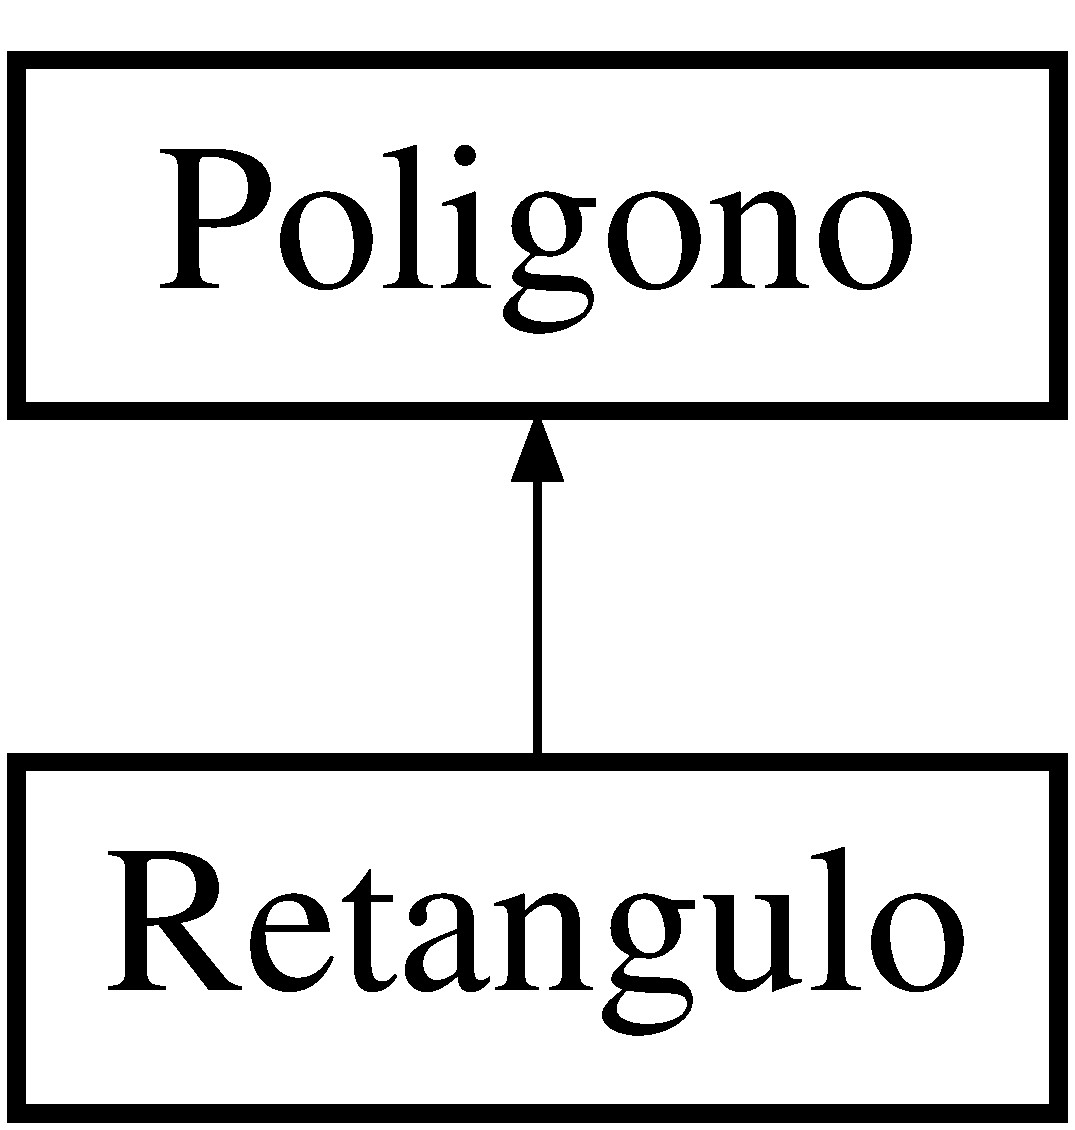
\includegraphics[height=2.000000cm]{class_poligono}
\end{center}
\end{figure}
\subsection*{Public Member Functions}
\begin{DoxyCompactItemize}
\item 
\mbox{\hyperlink{class_poligono_a9311a9a1496878c09c8508b3636e2870}{Poligono}} ()
\begin{DoxyCompactList}\small\item\em \mbox{\hyperlink{class_poligono}{Poligono}} é o Construtor da classe \mbox{\hyperlink{class_poligono}{Poligono}}. \end{DoxyCompactList}\item 
\mbox{\hyperlink{class_poligono_a4dd7136ee506cb4355cbdc724c55a4a0}{$\sim$\+Poligono}} ()
\item 
void \mbox{\hyperlink{class_poligono_a8cfc6f93c72f6ac5119a76cd339fc4c3}{insere\+Vertice}} (float mx, float my)
\begin{DoxyCompactList}\small\item\em insere\+Vertice é a função que insere os Vertices do \mbox{\hyperlink{class_poligono}{Poligono}} \end{DoxyCompactList}\item 
void \mbox{\hyperlink{class_poligono_a87d58f9d4827793eaa811491cce097b0}{imprime\+Poligono}} ()
\begin{DoxyCompactList}\small\item\em imprime\+Poligono é a função que imprime todos os pontos do poligono. \end{DoxyCompactList}\item 
float \mbox{\hyperlink{class_poligono_a29464a68eb3f3c00bb03f3f467d459c9}{rec\+Vertice}} ()
\begin{DoxyCompactList}\small\item\em rec\+Vertice é a função que recupera a quantidade de Vertices no \mbox{\hyperlink{class_poligono}{Poligono}} \end{DoxyCompactList}\item 
float \mbox{\hyperlink{class_poligono_ac1e37e274f61dff6c421f972ef1cf891}{area\+Poligono}} ()
\begin{DoxyCompactList}\small\item\em area\+Poligono é a Função que calcula a Área do \mbox{\hyperlink{class_poligono}{Poligono}}. \end{DoxyCompactList}\item 
void \mbox{\hyperlink{class_poligono_a4d757f52ba9366ab13537fb19b363e1e}{translada\+Poligono}} (float a, float b)
\begin{DoxyCompactList}\small\item\em translada\+Poligono é a Função que translada os pontos do poligono para (x+a) e (y+b) \end{DoxyCompactList}\item 
void \mbox{\hyperlink{class_poligono_a8dbf52a0e4da176f014062f9ec0fbafa}{rot\+Poligono}} (float ang, \mbox{\hyperlink{class_point}{Point}} p1)
\begin{DoxyCompactList}\small\item\em rot\+Poligono é a função que rotaciona o poligono em θ graus no sentido anti-\/horário em torno de um ponto (x0,y0) fornecido pelo usuário. \end{DoxyCompactList}\end{DoxyCompactItemize}
\subsection*{Protected Attributes}
\begin{DoxyCompactItemize}
\item 
\mbox{\hyperlink{class_point}{Point}} \mbox{\hyperlink{class_poligono_a5912ffab7b68ee4ac18660b9ea00b5ed}{p}} \mbox{[}100\mbox{]}
\item 
int \mbox{\hyperlink{class_poligono_a9ee4bec594127166d10a527298addc53}{N}}
\end{DoxyCompactItemize}


\subsection{Detailed Description}
The \mbox{\hyperlink{class_poligono}{Poligono}} class é usado para representar polígonos convexos. 

\subsection{Constructor \& Destructor Documentation}
\mbox{\Hypertarget{class_poligono_a9311a9a1496878c09c8508b3636e2870}\label{class_poligono_a9311a9a1496878c09c8508b3636e2870}} 
\index{Poligono@{Poligono}!Poligono@{Poligono}}
\index{Poligono@{Poligono}!Poligono@{Poligono}}
\subsubsection{\texorpdfstring{Poligono()}{Poligono()}}
{\footnotesize\ttfamily Poligono\+::\+Poligono (\begin{DoxyParamCaption}{ }\end{DoxyParamCaption})}



\mbox{\hyperlink{class_poligono}{Poligono}} é o Construtor da classe \mbox{\hyperlink{class_poligono}{Poligono}}. 

\mbox{\Hypertarget{class_poligono_a4dd7136ee506cb4355cbdc724c55a4a0}\label{class_poligono_a4dd7136ee506cb4355cbdc724c55a4a0}} 
\index{Poligono@{Poligono}!````~Poligono@{$\sim$\+Poligono}}
\index{````~Poligono@{$\sim$\+Poligono}!Poligono@{Poligono}}
\subsubsection{\texorpdfstring{$\sim$\+Poligono()}{~Poligono()}}
{\footnotesize\ttfamily Poligono\+::$\sim$\+Poligono (\begin{DoxyParamCaption}{ }\end{DoxyParamCaption})}



\subsection{Member Function Documentation}
\mbox{\Hypertarget{class_poligono_ac1e37e274f61dff6c421f972ef1cf891}\label{class_poligono_ac1e37e274f61dff6c421f972ef1cf891}} 
\index{Poligono@{Poligono}!area\+Poligono@{area\+Poligono}}
\index{area\+Poligono@{area\+Poligono}!Poligono@{Poligono}}
\subsubsection{\texorpdfstring{area\+Poligono()}{areaPoligono()}}
{\footnotesize\ttfamily float Poligono\+::area\+Poligono (\begin{DoxyParamCaption}{ }\end{DoxyParamCaption})}



area\+Poligono é a Função que calcula a Área do \mbox{\hyperlink{class_poligono}{Poligono}}. 

\begin{DoxyReturn}{Returns}
retorna a área do poligono. 
\end{DoxyReturn}
\mbox{\Hypertarget{class_poligono_a87d58f9d4827793eaa811491cce097b0}\label{class_poligono_a87d58f9d4827793eaa811491cce097b0}} 
\index{Poligono@{Poligono}!imprime\+Poligono@{imprime\+Poligono}}
\index{imprime\+Poligono@{imprime\+Poligono}!Poligono@{Poligono}}
\subsubsection{\texorpdfstring{imprime\+Poligono()}{imprimePoligono()}}
{\footnotesize\ttfamily void Poligono\+::imprime\+Poligono (\begin{DoxyParamCaption}{ }\end{DoxyParamCaption})}



imprime\+Poligono é a função que imprime todos os pontos do poligono. 

\mbox{\Hypertarget{class_poligono_a8cfc6f93c72f6ac5119a76cd339fc4c3}\label{class_poligono_a8cfc6f93c72f6ac5119a76cd339fc4c3}} 
\index{Poligono@{Poligono}!insere\+Vertice@{insere\+Vertice}}
\index{insere\+Vertice@{insere\+Vertice}!Poligono@{Poligono}}
\subsubsection{\texorpdfstring{insere\+Vertice()}{insereVertice()}}
{\footnotesize\ttfamily void Poligono\+::insere\+Vertice (\begin{DoxyParamCaption}\item[{float}]{mx,  }\item[{float}]{my }\end{DoxyParamCaption})}



insere\+Vertice é a função que insere os Vertices do \mbox{\hyperlink{class_poligono}{Poligono}} 


\begin{DoxyParams}{Parameters}
{\em mx} & Parametro para a coordenada X do ponto. \\
\hline
{\em my} & Paramentro para a coordenada y do ponto. \\
\hline
\end{DoxyParams}
\mbox{\Hypertarget{class_poligono_a29464a68eb3f3c00bb03f3f467d459c9}\label{class_poligono_a29464a68eb3f3c00bb03f3f467d459c9}} 
\index{Poligono@{Poligono}!rec\+Vertice@{rec\+Vertice}}
\index{rec\+Vertice@{rec\+Vertice}!Poligono@{Poligono}}
\subsubsection{\texorpdfstring{rec\+Vertice()}{recVertice()}}
{\footnotesize\ttfamily float Poligono\+::rec\+Vertice (\begin{DoxyParamCaption}{ }\end{DoxyParamCaption})}



rec\+Vertice é a função que recupera a quantidade de Vertices no \mbox{\hyperlink{class_poligono}{Poligono}} 

\begin{DoxyReturn}{Returns}
retorna o numero de vertices. 
\end{DoxyReturn}
\mbox{\Hypertarget{class_poligono_a8dbf52a0e4da176f014062f9ec0fbafa}\label{class_poligono_a8dbf52a0e4da176f014062f9ec0fbafa}} 
\index{Poligono@{Poligono}!rot\+Poligono@{rot\+Poligono}}
\index{rot\+Poligono@{rot\+Poligono}!Poligono@{Poligono}}
\subsubsection{\texorpdfstring{rot\+Poligono()}{rotPoligono()}}
{\footnotesize\ttfamily void Poligono\+::rot\+Poligono (\begin{DoxyParamCaption}\item[{float}]{ang,  }\item[{\mbox{\hyperlink{class_point}{Point}}}]{p1 }\end{DoxyParamCaption})}



rot\+Poligono é a função que rotaciona o poligono em θ graus no sentido anti-\/horário em torno de um ponto (x0,y0) fornecido pelo usuário. 


\begin{DoxyParams}{Parameters}
{\em ang} & é o paramentro do angulo \\
\hline
{\em p1} & é o ponto passado pelo usuario. \\
\hline
\end{DoxyParams}
\mbox{\Hypertarget{class_poligono_a4d757f52ba9366ab13537fb19b363e1e}\label{class_poligono_a4d757f52ba9366ab13537fb19b363e1e}} 
\index{Poligono@{Poligono}!translada\+Poligono@{translada\+Poligono}}
\index{translada\+Poligono@{translada\+Poligono}!Poligono@{Poligono}}
\subsubsection{\texorpdfstring{translada\+Poligono()}{transladaPoligono()}}
{\footnotesize\ttfamily void Poligono\+::translada\+Poligono (\begin{DoxyParamCaption}\item[{float}]{a,  }\item[{float}]{b }\end{DoxyParamCaption})}



translada\+Poligono é a Função que translada os pontos do poligono para (x+a) e (y+b) 


\begin{DoxyParams}{Parameters}
{\em a} & parametro para transladar a coordenada x dos pontos. \\
\hline
{\em b} & parametro para transladar a coordenada y dos pontos. \\
\hline
\end{DoxyParams}


\subsection{Member Data Documentation}
\mbox{\Hypertarget{class_poligono_a9ee4bec594127166d10a527298addc53}\label{class_poligono_a9ee4bec594127166d10a527298addc53}} 
\index{Poligono@{Poligono}!N@{N}}
\index{N@{N}!Poligono@{Poligono}}
\subsubsection{\texorpdfstring{N}{N}}
{\footnotesize\ttfamily int Poligono\+::N\hspace{0.3cm}{\ttfamily [protected]}}

\mbox{\Hypertarget{class_poligono_a5912ffab7b68ee4ac18660b9ea00b5ed}\label{class_poligono_a5912ffab7b68ee4ac18660b9ea00b5ed}} 
\index{Poligono@{Poligono}!p@{p}}
\index{p@{p}!Poligono@{Poligono}}
\subsubsection{\texorpdfstring{p}{p}}
{\footnotesize\ttfamily \mbox{\hyperlink{class_point}{Point}} Poligono\+::p\mbox{[}100\mbox{]}\hspace{0.3cm}{\ttfamily [protected]}}



The documentation for this class was generated from the following files\+:\begin{DoxyCompactItemize}
\item 
\mbox{\hyperlink{poligono_8h}{poligono.\+h}}\item 
\mbox{\hyperlink{poligono_8cpp}{poligono.\+cpp}}\end{DoxyCompactItemize}

\hypertarget{class_retangulo}{}\section{Retangulo Class Reference}
\label{class_retangulo}\index{Retangulo@{Retangulo}}


The \mbox{\hyperlink{class_retangulo}{Retangulo}} class é uma subclasse da Class \mbox{\hyperlink{class_poligono}{Poligono}}.  




{\ttfamily \#include $<$retangulo.\+h$>$}

Inheritance diagram for Retangulo\+:\begin{figure}[H]
\begin{center}
\leavevmode
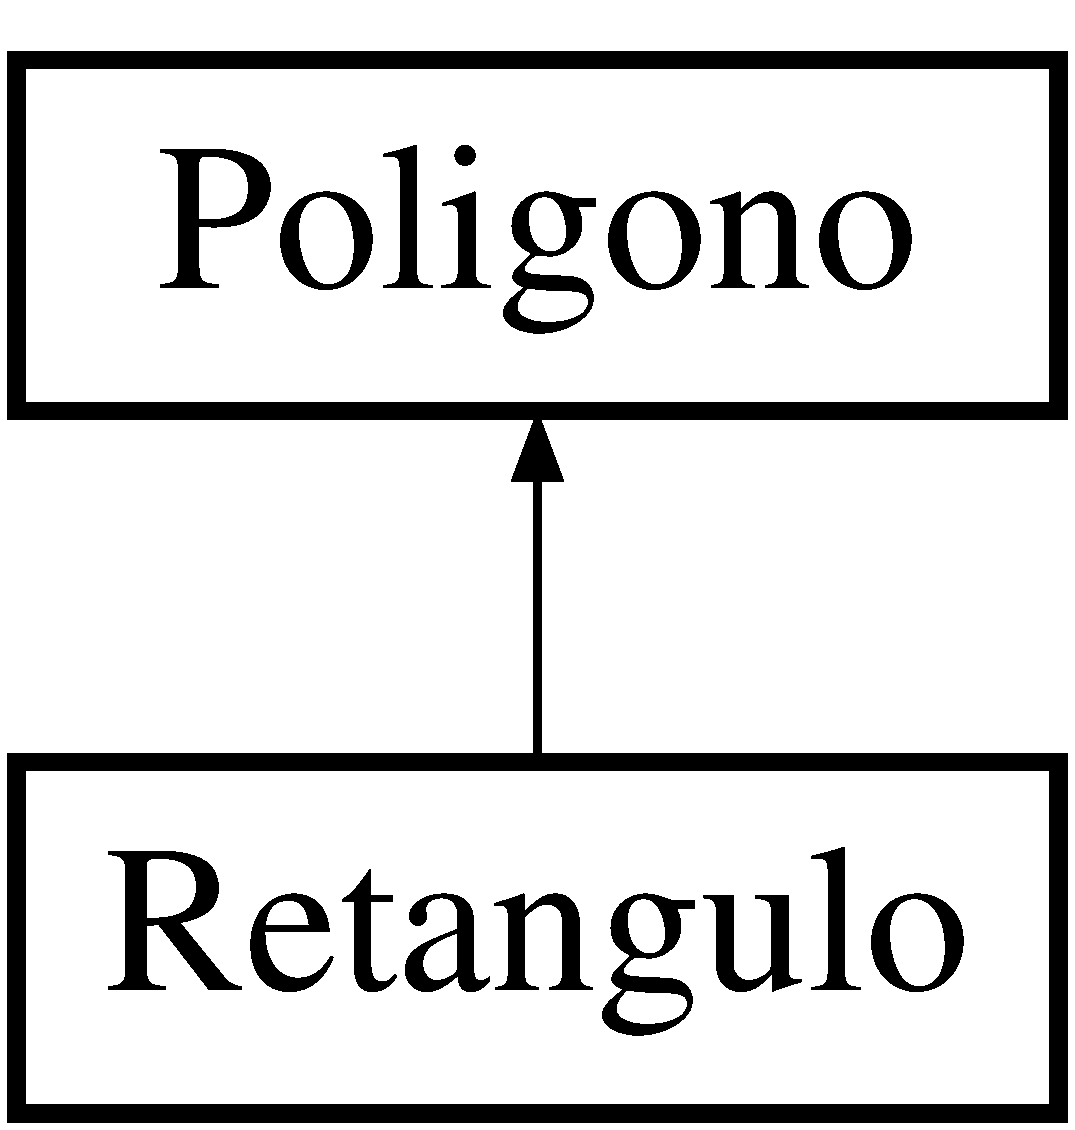
\includegraphics[height=2.000000cm]{class_retangulo}
\end{center}
\end{figure}
\subsection*{Public Member Functions}
\begin{DoxyCompactItemize}
\item 
\mbox{\hyperlink{class_retangulo_acca1dd211eefc8dc04658c943c0d1122}{Retangulo}} (float x, float y, float largura, float altura)
\begin{DoxyCompactList}\small\item\em \mbox{\hyperlink{class_retangulo}{Retangulo}} é o Construtor da Classe \mbox{\hyperlink{class_retangulo}{Retangulo}}. \end{DoxyCompactList}\item 
\mbox{\hyperlink{class_point}{Point}} \mbox{\hyperlink{class_retangulo_a0f6df53839be4fab7ffef3172481dcb6}{Enc\+Centro\+Massa\+Ret}} (\mbox{\hyperlink{class_retangulo}{Retangulo}} \&mr)
\begin{DoxyCompactList}\small\item\em Enc\+Centro\+Massa\+Ret é a função que encontra o centro de massa do retangulo. \end{DoxyCompactList}\end{DoxyCompactItemize}
\subsection*{Additional Inherited Members}


\subsection{Detailed Description}
The \mbox{\hyperlink{class_retangulo}{Retangulo}} class é uma subclasse da Class \mbox{\hyperlink{class_poligono}{Poligono}}. 

\subsection{Constructor \& Destructor Documentation}
\mbox{\Hypertarget{class_retangulo_acca1dd211eefc8dc04658c943c0d1122}\label{class_retangulo_acca1dd211eefc8dc04658c943c0d1122}} 
\index{Retangulo@{Retangulo}!Retangulo@{Retangulo}}
\index{Retangulo@{Retangulo}!Retangulo@{Retangulo}}
\subsubsection{\texorpdfstring{Retangulo()}{Retangulo()}}
{\footnotesize\ttfamily Retangulo\+::\+Retangulo (\begin{DoxyParamCaption}\item[{float}]{x,  }\item[{float}]{y,  }\item[{float}]{largura,  }\item[{float}]{altura }\end{DoxyParamCaption})}



\mbox{\hyperlink{class_retangulo}{Retangulo}} é o Construtor da Classe \mbox{\hyperlink{class_retangulo}{Retangulo}}. 


\begin{DoxyParams}{Parameters}
{\em x} & paramentro da coordenada x do ponto da posição superior esquerda \\
\hline
{\em y} & paramentro da coordenada y do ponto da posição superior esquerda \\
\hline
{\em largura} & é a largura do \mbox{\hyperlink{class_retangulo}{Retangulo}} \\
\hline
{\em altura} & é a altura do \mbox{\hyperlink{class_retangulo}{Retangulo}} \\
\hline
\end{DoxyParams}


\subsection{Member Function Documentation}
\mbox{\Hypertarget{class_retangulo_a0f6df53839be4fab7ffef3172481dcb6}\label{class_retangulo_a0f6df53839be4fab7ffef3172481dcb6}} 
\index{Retangulo@{Retangulo}!Enc\+Centro\+Massa\+Ret@{Enc\+Centro\+Massa\+Ret}}
\index{Enc\+Centro\+Massa\+Ret@{Enc\+Centro\+Massa\+Ret}!Retangulo@{Retangulo}}
\subsubsection{\texorpdfstring{Enc\+Centro\+Massa\+Ret()}{EncCentroMassaRet()}}
{\footnotesize\ttfamily \mbox{\hyperlink{class_point}{Point}} Retangulo\+::\+Enc\+Centro\+Massa\+Ret (\begin{DoxyParamCaption}\item[{\mbox{\hyperlink{class_retangulo}{Retangulo}} \&}]{mr }\end{DoxyParamCaption})}



Enc\+Centro\+Massa\+Ret é a função que encontra o centro de massa do retangulo. 

\begin{DoxyReturn}{Returns}
Retorna o ponto onde se encontra o centro de massa. 
\end{DoxyReturn}


The documentation for this class was generated from the following files\+:\begin{DoxyCompactItemize}
\item 
\mbox{\hyperlink{retangulo_8h}{retangulo.\+h}}\item 
\mbox{\hyperlink{retangulo_8cpp}{retangulo.\+cpp}}\end{DoxyCompactItemize}

\chapter{File Documentation}
\hypertarget{main_8cpp}{}\section{main.\+cpp File Reference}
\label{main_8cpp}\index{main.\+cpp@{main.\+cpp}}
{\ttfamily \#include $<$iostream$>$}\newline
{\ttfamily \#include \char`\"{}point.\+h\char`\"{}}\newline
\subsection*{Functions}
\begin{DoxyCompactItemize}
\item 
int \mbox{\hyperlink{main_8cpp_ae66f6b31b5ad750f1fe042a706a4e3d4}{main}} ()
\end{DoxyCompactItemize}


\subsection{Function Documentation}
\mbox{\Hypertarget{main_8cpp_ae66f6b31b5ad750f1fe042a706a4e3d4}\label{main_8cpp_ae66f6b31b5ad750f1fe042a706a4e3d4}} 
\index{main.\+cpp@{main.\+cpp}!main@{main}}
\index{main@{main}!main.\+cpp@{main.\+cpp}}
\subsubsection{\texorpdfstring{main()}{main()}}
{\footnotesize\ttfamily int main (\begin{DoxyParamCaption}{ }\end{DoxyParamCaption})}


\hypertarget{point_8cpp}{}\section{point.\+cpp File Reference}
\label{point_8cpp}\index{point.\+cpp@{point.\+cpp}}
{\ttfamily \#include \char`\"{}point.\+h\char`\"{}}\newline
{\ttfamily \#include $<$iostream$>$}\newline
{\ttfamily \#include $<$cmath$>$}\newline
\subsection*{Macros}
\begin{DoxyCompactItemize}
\item 
\#define \mbox{\hyperlink{point_8cpp_a1daf785e3f68d293c7caa1c756d5cb74}{pi}}~3.\+1415
\end{DoxyCompactItemize}


\subsection{Macro Definition Documentation}
\mbox{\Hypertarget{point_8cpp_a1daf785e3f68d293c7caa1c756d5cb74}\label{point_8cpp_a1daf785e3f68d293c7caa1c756d5cb74}} 
\index{point.\+cpp@{point.\+cpp}!pi@{pi}}
\index{pi@{pi}!point.\+cpp@{point.\+cpp}}
\subsubsection{\texorpdfstring{pi}{pi}}
{\footnotesize\ttfamily \#define pi~3.\+1415}


\hypertarget{point_8h}{}\section{point.\+h File Reference}
\label{point_8h}\index{point.\+h@{point.\+h}}
\subsection*{Classes}
\begin{DoxyCompactItemize}
\item 
class \mbox{\hyperlink{class_point}{Point}}
\begin{DoxyCompactList}\small\item\em The \mbox{\hyperlink{class_point}{Point}} class é usada para criar Pontos em um Plano Bidimensional. \end{DoxyCompactList}\end{DoxyCompactItemize}

\hypertarget{poligono_8cpp}{}\section{poligono.\+cpp File Reference}
\label{poligono_8cpp}\index{poligono.\+cpp@{poligono.\+cpp}}
{\ttfamily \#include \char`\"{}poligono.\+h\char`\"{}}\newline
{\ttfamily \#include $<$iostream$>$}\newline
{\ttfamily \#include $<$cmath$>$}\newline

\hypertarget{poligono_8h}{}\section{poligono.\+h File Reference}
\label{poligono_8h}\index{poligono.\+h@{poligono.\+h}}
{\ttfamily \#include \char`\"{}point.\+h\char`\"{}}\newline
\subsection*{Classes}
\begin{DoxyCompactItemize}
\item 
class \mbox{\hyperlink{class_poligono}{Poligono}}
\begin{DoxyCompactList}\small\item\em The \mbox{\hyperlink{class_poligono}{Poligono}} class é usado para representar polígonos convexos. \end{DoxyCompactList}\end{DoxyCompactItemize}

\hypertarget{_r_e_a_d_m_e_8md}{}\section{R\+E\+A\+D\+M\+E.\+md File Reference}
\label{_r_e_a_d_m_e_8md}\index{R\+E\+A\+D\+M\+E.\+md@{R\+E\+A\+D\+M\+E.\+md}}

\hypertarget{retangulo_8cpp}{}\section{retangulo.\+cpp File Reference}
\label{retangulo_8cpp}\index{retangulo.\+cpp@{retangulo.\+cpp}}
{\ttfamily \#include \char`\"{}retangulo.\+h\char`\"{}}\newline
{\ttfamily \#include $<$iostream$>$}\newline

\hypertarget{retangulo_8h}{}\section{retangulo.\+h File Reference}
\label{retangulo_8h}\index{retangulo.\+h@{retangulo.\+h}}
{\ttfamily \#include \char`\"{}poligono.\+h\char`\"{}}\newline
\subsection*{Classes}
\begin{DoxyCompactItemize}
\item 
class \mbox{\hyperlink{class_retangulo}{Retangulo}}
\begin{DoxyCompactList}\small\item\em The \mbox{\hyperlink{class_retangulo}{Retangulo}} class é uma subclasse da Class \mbox{\hyperlink{class_poligono}{Poligono}}. \end{DoxyCompactList}\end{DoxyCompactItemize}

%--- End generated contents ---

% Index
\backmatter
\newpage
\phantomsection
\clearemptydoublepage
\addcontentsline{toc}{chapter}{Index}
\printindex

\end{document}
